%!TEX root = ../main.tex

\chapter{Validación experimental}
\label{ch:validacion}

Una vez acabadas individualmente todas las partes del proyecto, el hardware
(\cref{ch:hardware}), el firmware (\cref{ch:firmware}) y el software del PFD
(\cref{ch:software}), en este capítulo se integran todos los subsistemas y se
comprueba el cumplimiento de los requisitos definidos.

La validación se organiza en tres bloques. Primero se verifica que el hardware es
correcto a nivel eléctrico, ampliando lo expuesto en la \cref{sec:verificacion}. A
continuación se comprueba que el sistema cubre las funciones requeridas. Por último
se cuantifican las magnitudes de rendimiento: la precisión de actitud, la latencia,
las tasas de actualización, etc.


% ========================================================================
\section{Validación del hardware}
\label{sec:val_hardware}

Antes de realizar las comprobaciones de requisitos con el sistema completo se
verifica el comportamiento eléctrico de la placa. Para ello se analizan tres puntos
concretos: la estabilidad de los raíles de alimentación bajo la carga real a la que
estará sometida, el consumo de corriente del sistema y la integridad de los buses,
en concreto el bus I2C. Estas medidas se toman con el sistema en régimen de
transmisión, con la radio emitiendo a \SI{20}{\hertz} y el resto de sensores
activos, que es la condición de mayor consumo y de mayor actividad en los buses.

\subsection{Raíles de alimentación}
\label{sec:val_alim}

Con la placa alimentada por USB-C se miden con el osciloscopio los raíles de
\SI{3.3}{\volt} y \SI{5}{\volt}. Se hacen medidas conservando la componente de
continua (\cref{fig:val_rail_idle_5v,fig:val_rail_idle_3v3}) y eliminando dicha
componente para analizar el rizado
(\cref{fig:val_rail_tx_ldo,fig:val_rail_tx_ams,fig:val_rail_tx_5v}).

\begin{figure}[H]
    \centering
    \begin{subfigure}{0.48\linewidth}
        \centering
        \includegraphics[width=\linewidth]{Figures/png/DSO00002.png}
        \caption{Raíl de \SI{5}{\volt}.}
        \label{fig:val_rail_idle_5v}
    \end{subfigure}\hfill
    \begin{subfigure}{0.48\linewidth}
        \centering
        \includegraphics[width=\linewidth]{Figures/png/DSO00001.png}
        \caption{Raíl de \SI{3.3}{\volt}.}
        \label{fig:val_rail_idle_3v3}
    \end{subfigure}
    \caption{Raíles de alimentación en reposo, ambos en su valor nominal.}
    \label{fig:val_rail_idle}
\end{figure}

\begin{figure}[H]
    \centering
    \begin{subfigure}{0.48\linewidth}
        \centering
        \includegraphics[width=\linewidth]{Figures/png/DSO00009.png}
        \caption{\SI{3.3}{\volt}, LDO NJM12856DL3.}
        \label{fig:val_rail_tx_ldo}
    \end{subfigure}\hfill
    \begin{subfigure}{0.48\linewidth}
        \centering
        \includegraphics[width=\linewidth]{Figures/png/DSO00016.png}
        \caption{\SI{3.3}{\volt}, AMS1117 integrado.}
        \label{fig:val_rail_tx_ams}
    \end{subfigure}

    \vspace{0.6em}

    \begin{subfigure}{0.48\linewidth}
        \centering
        \includegraphics[width=\linewidth]{Figures/png/DSO00007.png}
        \caption{\SI{5}{\volt}, entrada sin regular.}
        \label{fig:val_rail_tx_5v}
    \end{subfigure}
    \caption{Rizado de los raíles bajo transmisión a \SI{20}{\hertz}. La salida
             del LDO~(\subref{fig:val_rail_tx_ldo}) presenta un rizado de pequeña
             amplitud, inferior al del regulador integrado
             AMS1117~(\subref{fig:val_rail_tx_ams}), que alimenta además la carga
             digital propia del ESP32. La comparación es indicativa y respalda el
             empleo de un regulador dedicado para el raíl sensible de RF y
             sensores. En el raíl de entrada de
             \SI{5}{\volt} sin regular~(\subref{fig:val_rail_tx_5v}) la
             perturbación de la radio es máxima.}
    \label{fig:val_rail_tx}
\end{figure}

Del análisis de las figuras con la componente continua no se pueden extraer conclusiones claras sobre la calidad de la señal, así que se analiza únicamente el rizado con la componente de alterna. Para empezar, la \cref{fig:val_rail_tx_5v} muestra el rizado del raíl de \SI{5}{\volt}. Se observa un rizado notable, ya que se mide el bus antes de pasar por ningún elemento regulador. Aun así, los valores de pico a pico son de \SI{60}{\milli\volt}, aceptables para esta aplicación. Lo más relevante de esta figura son los picos observables cada \SI{50}{\milli\second}, que coinciden con la frecuencia de envío de datos del transmisor y provocan una caída instantánea de corriente.

Las \cref{fig:val_rail_tx_ldo,fig:val_rail_tx_ams} pertenecen a los raíles de \SI{3.3}{\volt}: por un lado el del LDO dedicado, y por otro el del regulador que integra la placa del ESP32. Se observa que el LDO ofrece una calidad de señal mucho mejor, lo que justifica su uso frente al regulador del ESP32. En este raíl se aprecian los mismos picos de corriente que en el de \SI{5}{\volt}, pero, al haber condensadores de por medio, son muy inferiores en magnitud, casi imperceptibles. En conjunto, la calidad de la alimentación es buena.

\subsection{Consumo del sistema}
\label{sec:val_consumo}

El consumo de corriente del sistema completo se mide con un multímetro en serie
con la alimentación USB-C, con la placa en funcionamiento nominal y todos los sensores activos. Principalmente, esta medida sirve para determinar si se supera el límite de \SI{0.5}{\ampere} que fija el LDO; dado que el raíl de \SI{3.3}{\volt} se deriva del de \SI{5}{\volt}, la corriente de ese raíl es necesariamente menor que el consumo total. Se observa que el consumo medio en condiciones de uso nominal, con todos los sensores activos y el enlace de telemetría establecido, es de \SI{0.21}{\ampere}, muy por debajo del límite de \SI{0.5}{\ampere} del LDO, como se anticipó en el \cref{ch:hardware}.

El multímetro mide el consumo medio, no los picos instantáneos de la transmisión; estos transitorios de \SI{50}{\milli\second} se aprecian en el rizado de la \cref{fig:val_rail_tx} y quedan absorbidos por los condensadores de desacoplo, sin provocar reinicios. Tanto en la inicialización como, sobre todo, cuando el enlace pierde el receptor, el consumo medio sube hasta \SI{0.26}{\ampere}, sin superar el límite. Este aumento parece contraintuitivo en un principio, pero es consecuencia del mecanismo de reconocimiento automático (\textit{Enhanced ShockBurst}) del NRF24L01+: al perderse el enlace, el transmisor reintenta enviar cada paquete hasta agotar el número de retransmisiones configurado en el firmware, manteniendo así el amplificador de potencia activo durante más tiempo en cada ciclo. Esto permite verificar de forma indirecta el correcto funcionamiento del enlace.

\begin{table}[H]
    \centering
    \caption{Consumo total del sistema en distintos estados del enlace}
    \label{tab:val_consumo}
    \footnotesize
    \begin{tabularx}{\linewidth}{X C{3.0cm}}
        \toprule
        \textbf{Estado} & \textbf{Consumo total (\si{\ampere})} \\
        \midrule
        Transmisión nominal (enlace establecido)    & 0.21 \\
        Receptor desconectado (reintentos activos)   & 0.26 \\
        \bottomrule
    \end{tabularx}
\end{table}

\begin{figure}[H]
    \centering
    \begin{subfigure}{0.48\linewidth}
        \centering
        
        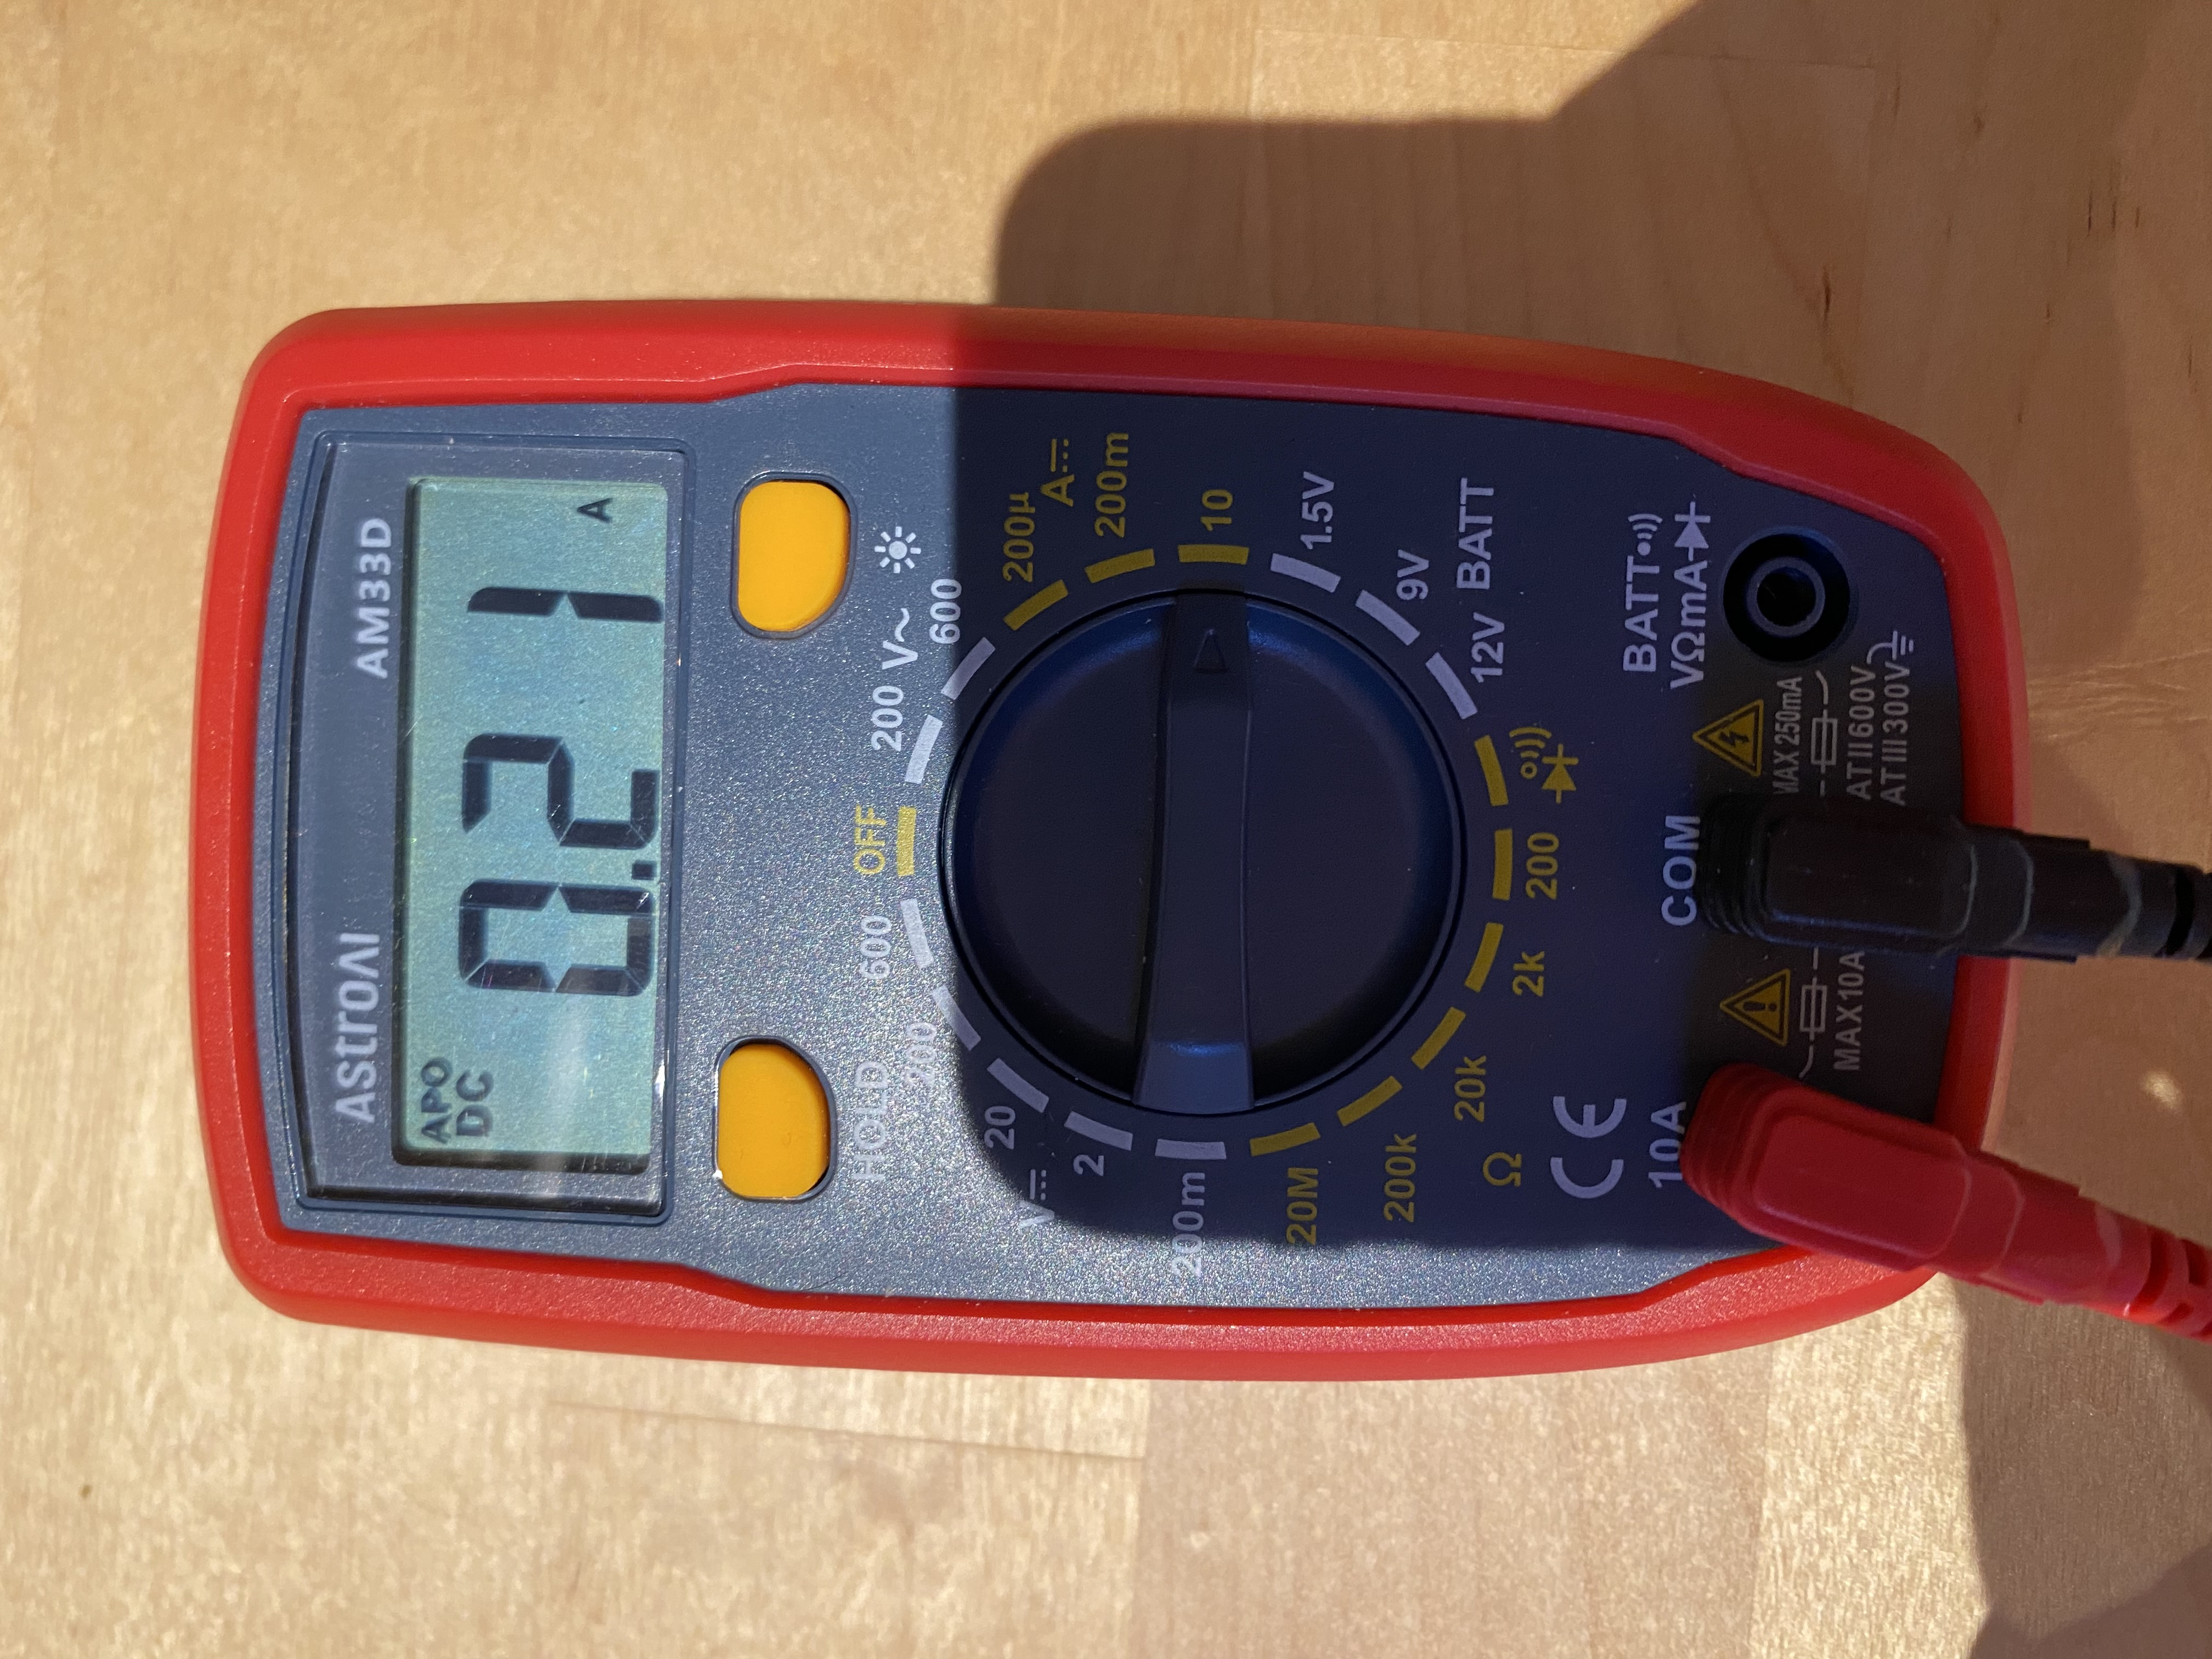
\includegraphics[width=\linewidth,angle=-90]{Figures/multi_21.jpeg}
        \caption{Consumo del sistema en condiciones nominales}
        \label{fig:multi_21}
    \end{subfigure}\hfill
    \begin{subfigure}{0.48\linewidth}
        \centering
        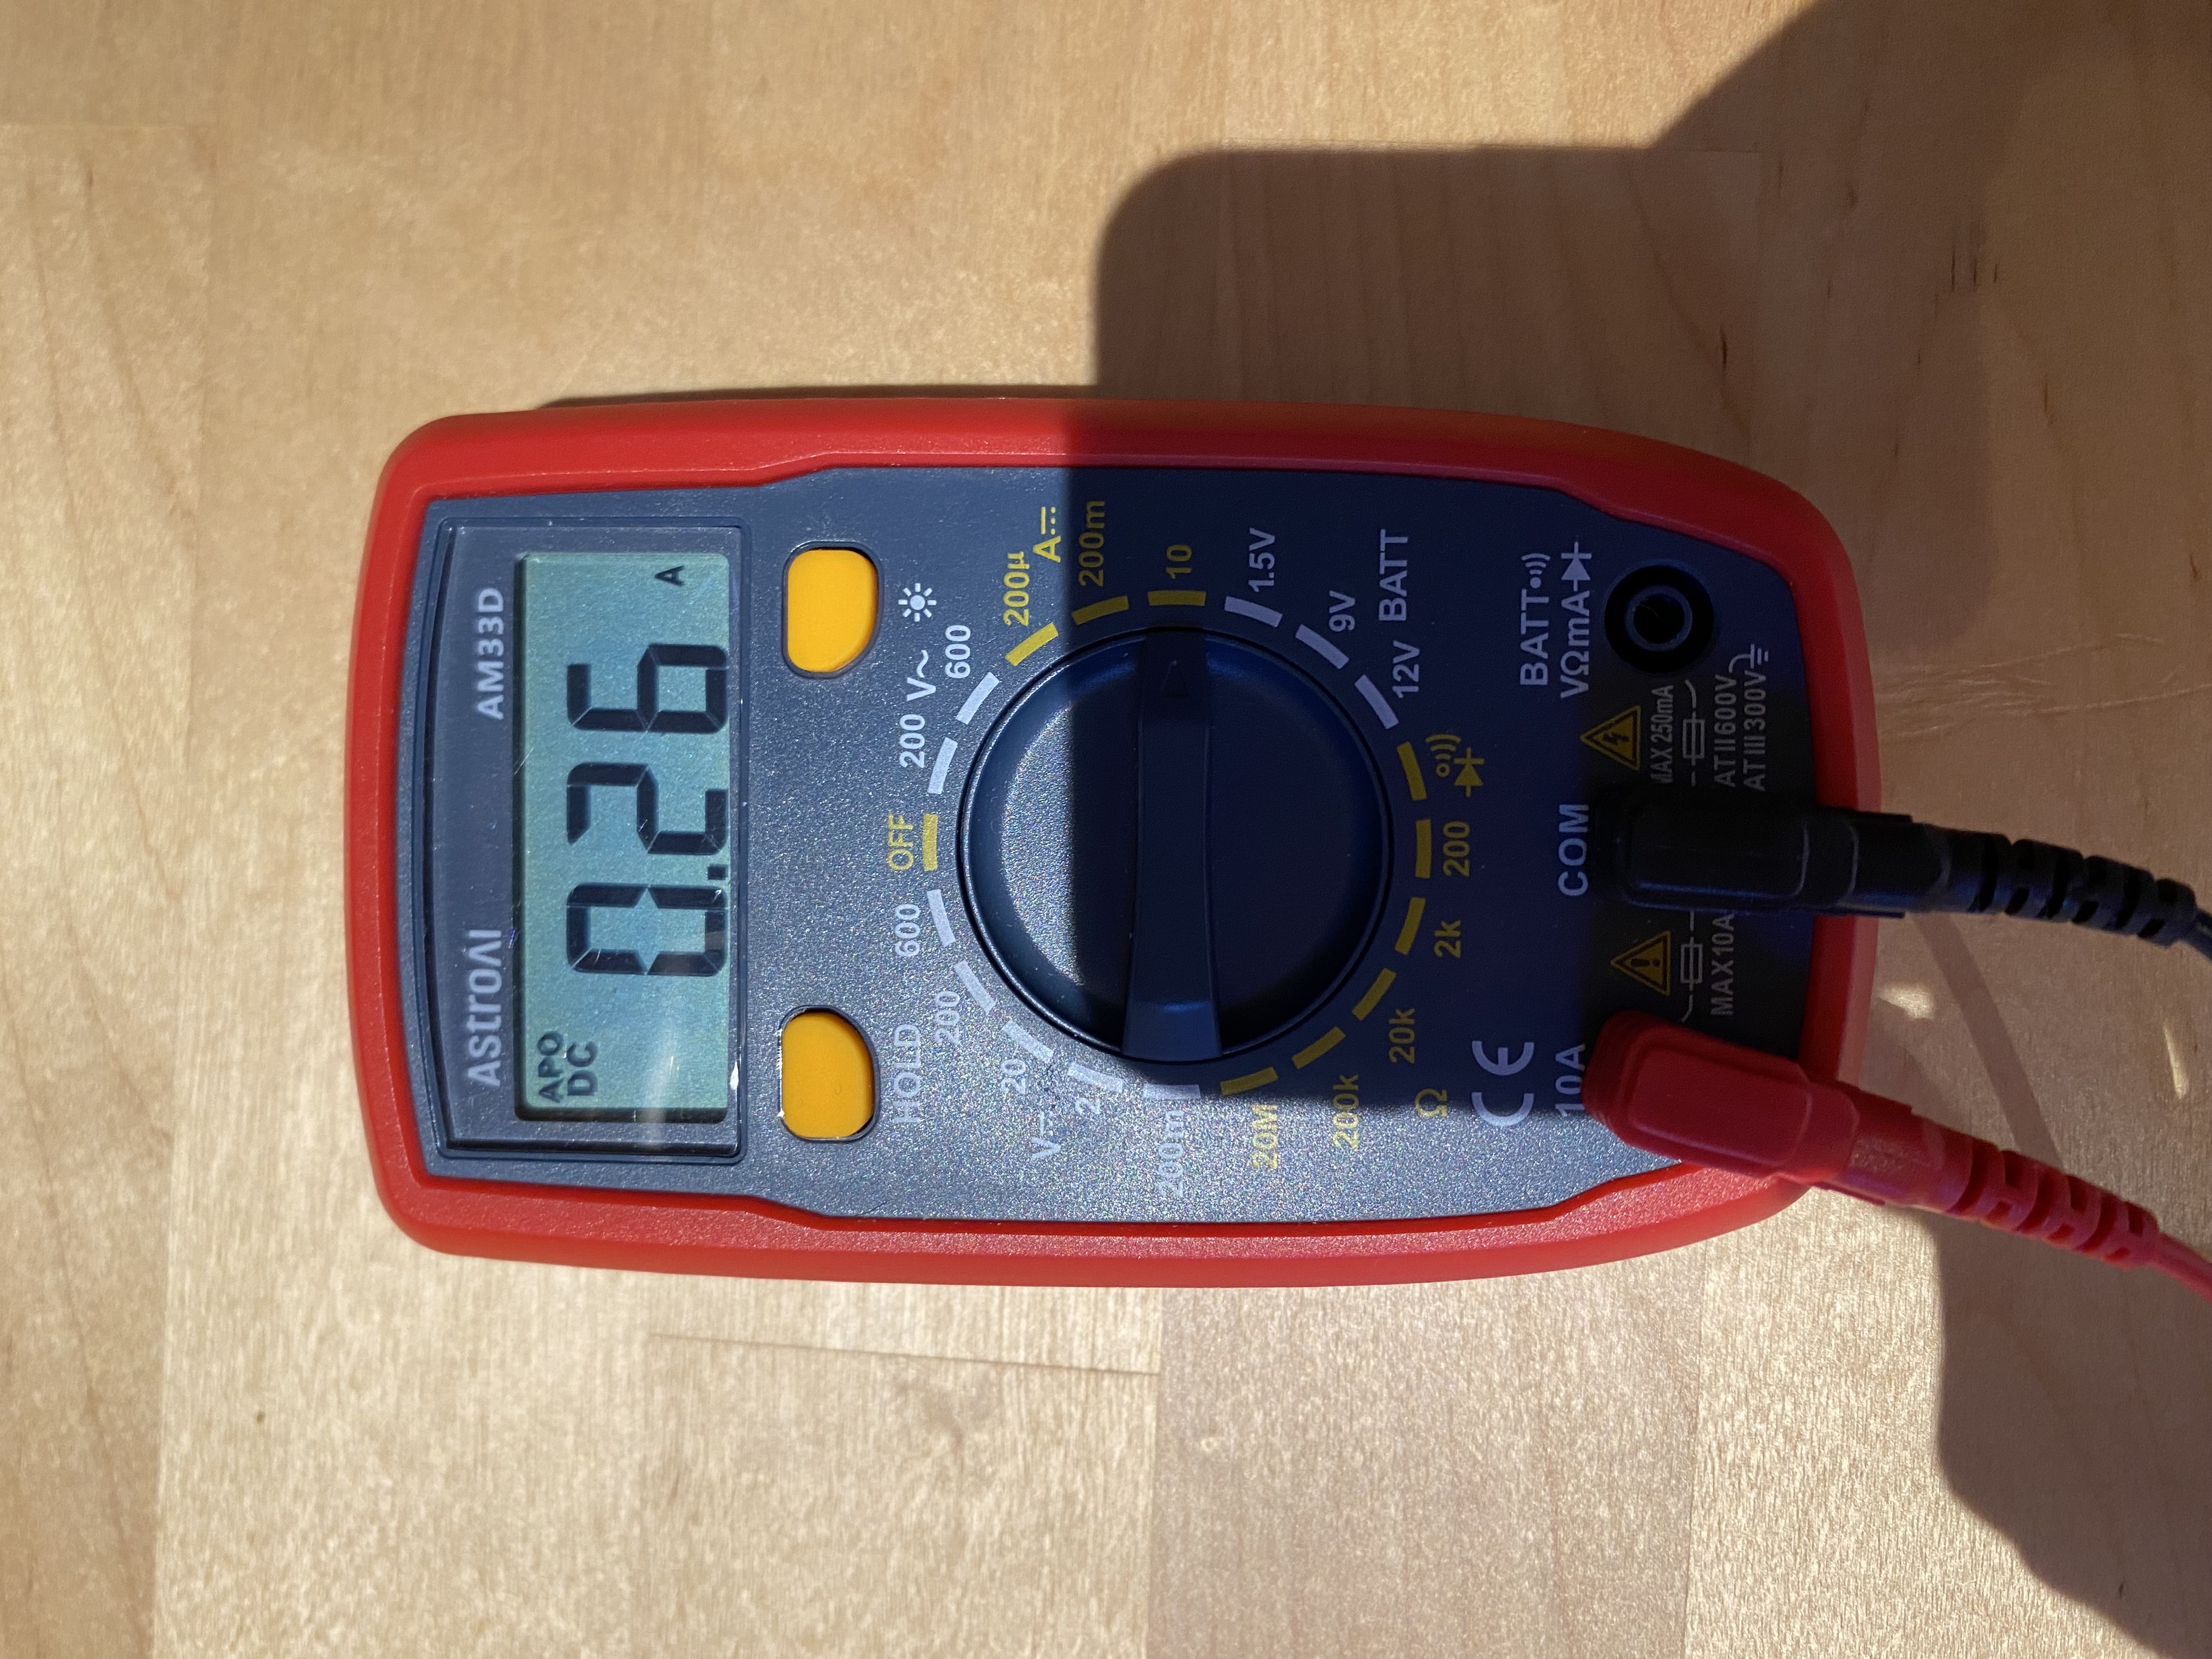
\includegraphics[width=\linewidth,angle=-90]{Figures/multi_26.jpeg}
        \caption{Consumo del sistema sin enlace de telemetría}
        \label{fig:multi_26}
    \end{subfigure}
    \caption{Consumo total del sistema medido con multímetro en serie con la
             alimentación USB-C: condiciones nominales y con el receptor
             desconectado.}
    \label{fig:val_consumo}
\end{figure}

\subsection{Integridad del bus I2C}
\label{sec:val_i2c}

Para verificar el bus I2C compartido por los tres sensores (MPU-9250, BMP280 y
VL53L1X) se capturan simultáneamente las líneas de reloj (SCL) y de datos (SDA)
durante el funcionamiento normal (\cref{fig:val_i2c}). El reloj presenta una
frecuencia de \SI{400}{\kilo\hertz}, coincidiendo con el valor configurado en la
\cref{sec:fw_imu}, y el bus opera de forma estable durante todo el funcionamiento,
sin pérdida de tramas ni errores de lectura de los sensores. Esto confirma en
operación lo indicado en la \cref{sec:bus_i2c}: el valor
equivalente de las resistencias de pull-up de los módulos es adecuado y el bus
opera sin problemas a la velocidad configurada.

\begin{figure}[H]
    \centering
    \includegraphics[width=0.7\linewidth]{Figures/png/DSO00014.png}
    \caption{Líneas SCL y SDA del bus I2C a \SI{400}{\kilo\hertz}.}
    \label{fig:val_i2c}
\end{figure}


% ========================================================================
\section{Validación funcional}
\label{sec:val_funcional}

Con el sistema completo integrado y en funcionamiento se comprueba que cada
requisito funcional queda cubierto. El nodo transmisor adquiere y fusiona los
datos, los codifica en ARINC 429 y los transmite. El receptor los decodifica y
los entrega al PC y el PFD los representa en disposición Basic-T. 

La \cref{tab:val_funcional} resume la comprobación de cada requisito funcional.

\begin{table}[H]
    \centering
    \caption{Comprobación de los requisitos funcionales}
    \label{tab:val_funcional}
    \footnotesize
    \begin{tabularx}{\linewidth}{l X l}
        \toprule
        \textbf{ID} & \textbf{Comprobación} & \textbf{Estado} \\
        \midrule
        RF01 & El horizonte artificial sigue el cabeceo y el alabeo de la placa en tiempo real. & Cumple \\
        RF02 & El indicador de rumbo refleja el rumbo magnético; precisión cuantificada en la \cref{sec:val_rumbo}. & Cumple \\
        RF03 & La cinta de altitud muestra la altitud MSL derivada de la presión barométrica. & Cumple \\
        RF04 & El VSI muestra la velocidad vertical estimada. & Cumple \\
        RF05 & La cinta de velocidad muestra la velocidad respecto al suelo del GNSS cuando hay \textit{fix}. & Cumple \\
        RF06 & El indicador de proximidad muestra la distancia al suelo (ToF como fuente activa). & Cumple \\
        RF07 & La telemetría llega del transmisor al receptor; enlace validado en la \cref{sec:val_enlace}. & Cumple \\
        RF08 & El receptor decodifica las palabras ARINC 429 por etiqueta y descarta las inválidas. & Cumple \\
        RF09 & El PFD se representa con la disposición Basic-T completa. & Cumple \\
        \bottomrule
    \end{tabularx}
\end{table}


% ========================================================================
\section{Precisión de la estimación de actitud}
\label{sec:val_actitud}

Para estudiar la precisión de la estimación de actitud, se evalúa esta magnitud en condiciones estáticas frente a ángulos de referencia conocidos. Para obtener estos ángulos se emplean escuadras de dibujo apoyadas sobre una superficie plana y nivelada, con las que se fijan las referencias de $30^{\circ}$, $45^{\circ}$ y $60^{\circ}$. Para cada ángulo se registra el valor de cabeceo (P) o alabeo (R) indicado por el PFD. Antes de tomar las medidas se han aplicado los \textit{offsets} de montaje de la \cref{tab:mahony_params}.

El montaje empleado se muestra en la \cref{fig:val_actitud_escuadra} y los valores obtenidos se recogen en la \cref{tab:val_actitud} (El resto de imagenes de las pruebas se encuentran en el Anexo III). El error máximo observado es de $1{,}8^{\circ}$, dentro del umbral de $3^{\circ}$ fijado por RP04.

\begin{table}[H]
    \centering
    \caption{Precisión de la estimación de actitud en condiciones estáticas}
    \label{tab:val_actitud}
    \footnotesize
    \begin{tabularx}{\linewidth}{C{2.6cm} C{2.4cm} C{2.0cm} C{2.4cm} C{2.0cm}}
        \toprule
        \textbf{Ref.\ ($^{\circ}$)} & \textbf{Cabeceo P ($^{\circ}$)} & \textbf{Error ($^{\circ}$)} & \textbf{Alabeo R ($^{\circ}$)} & \textbf{Error ($^{\circ}$)} \\
        \midrule
        $0$    & $-0{,}1$  & $0{,}1$ & $0{,}1$   & $0{,}1$ \\
        $+30$  & $28{,}9$  & $1{,}1$ & $29{,}1$  & $0{,}9$ \\
        $-30$  & $-29{,}9$ & $0{,}1$ & $-29{,}3$ & $0{,}7$ \\
        $+45$  & $43{,}4$  & $1{,}6$ & $43{,}8$  & $1{,}2$ \\
        $-45$  & $-44{,}4$ & $0{,}6$ & $-43{,}8$ & $1{,}2$ \\
        $+60$  & $58{,}2$  & $1{,}8$ & $58{,}5$  & $1{,}5$ \\
        $-60$  & $-59{,}1$ & $0{,}9$ & $-58{,}8$ & $1{,}2$ \\
        \bottomrule
    \end{tabularx}
\end{table}

\begin{figure}[H]
    \centering
    
    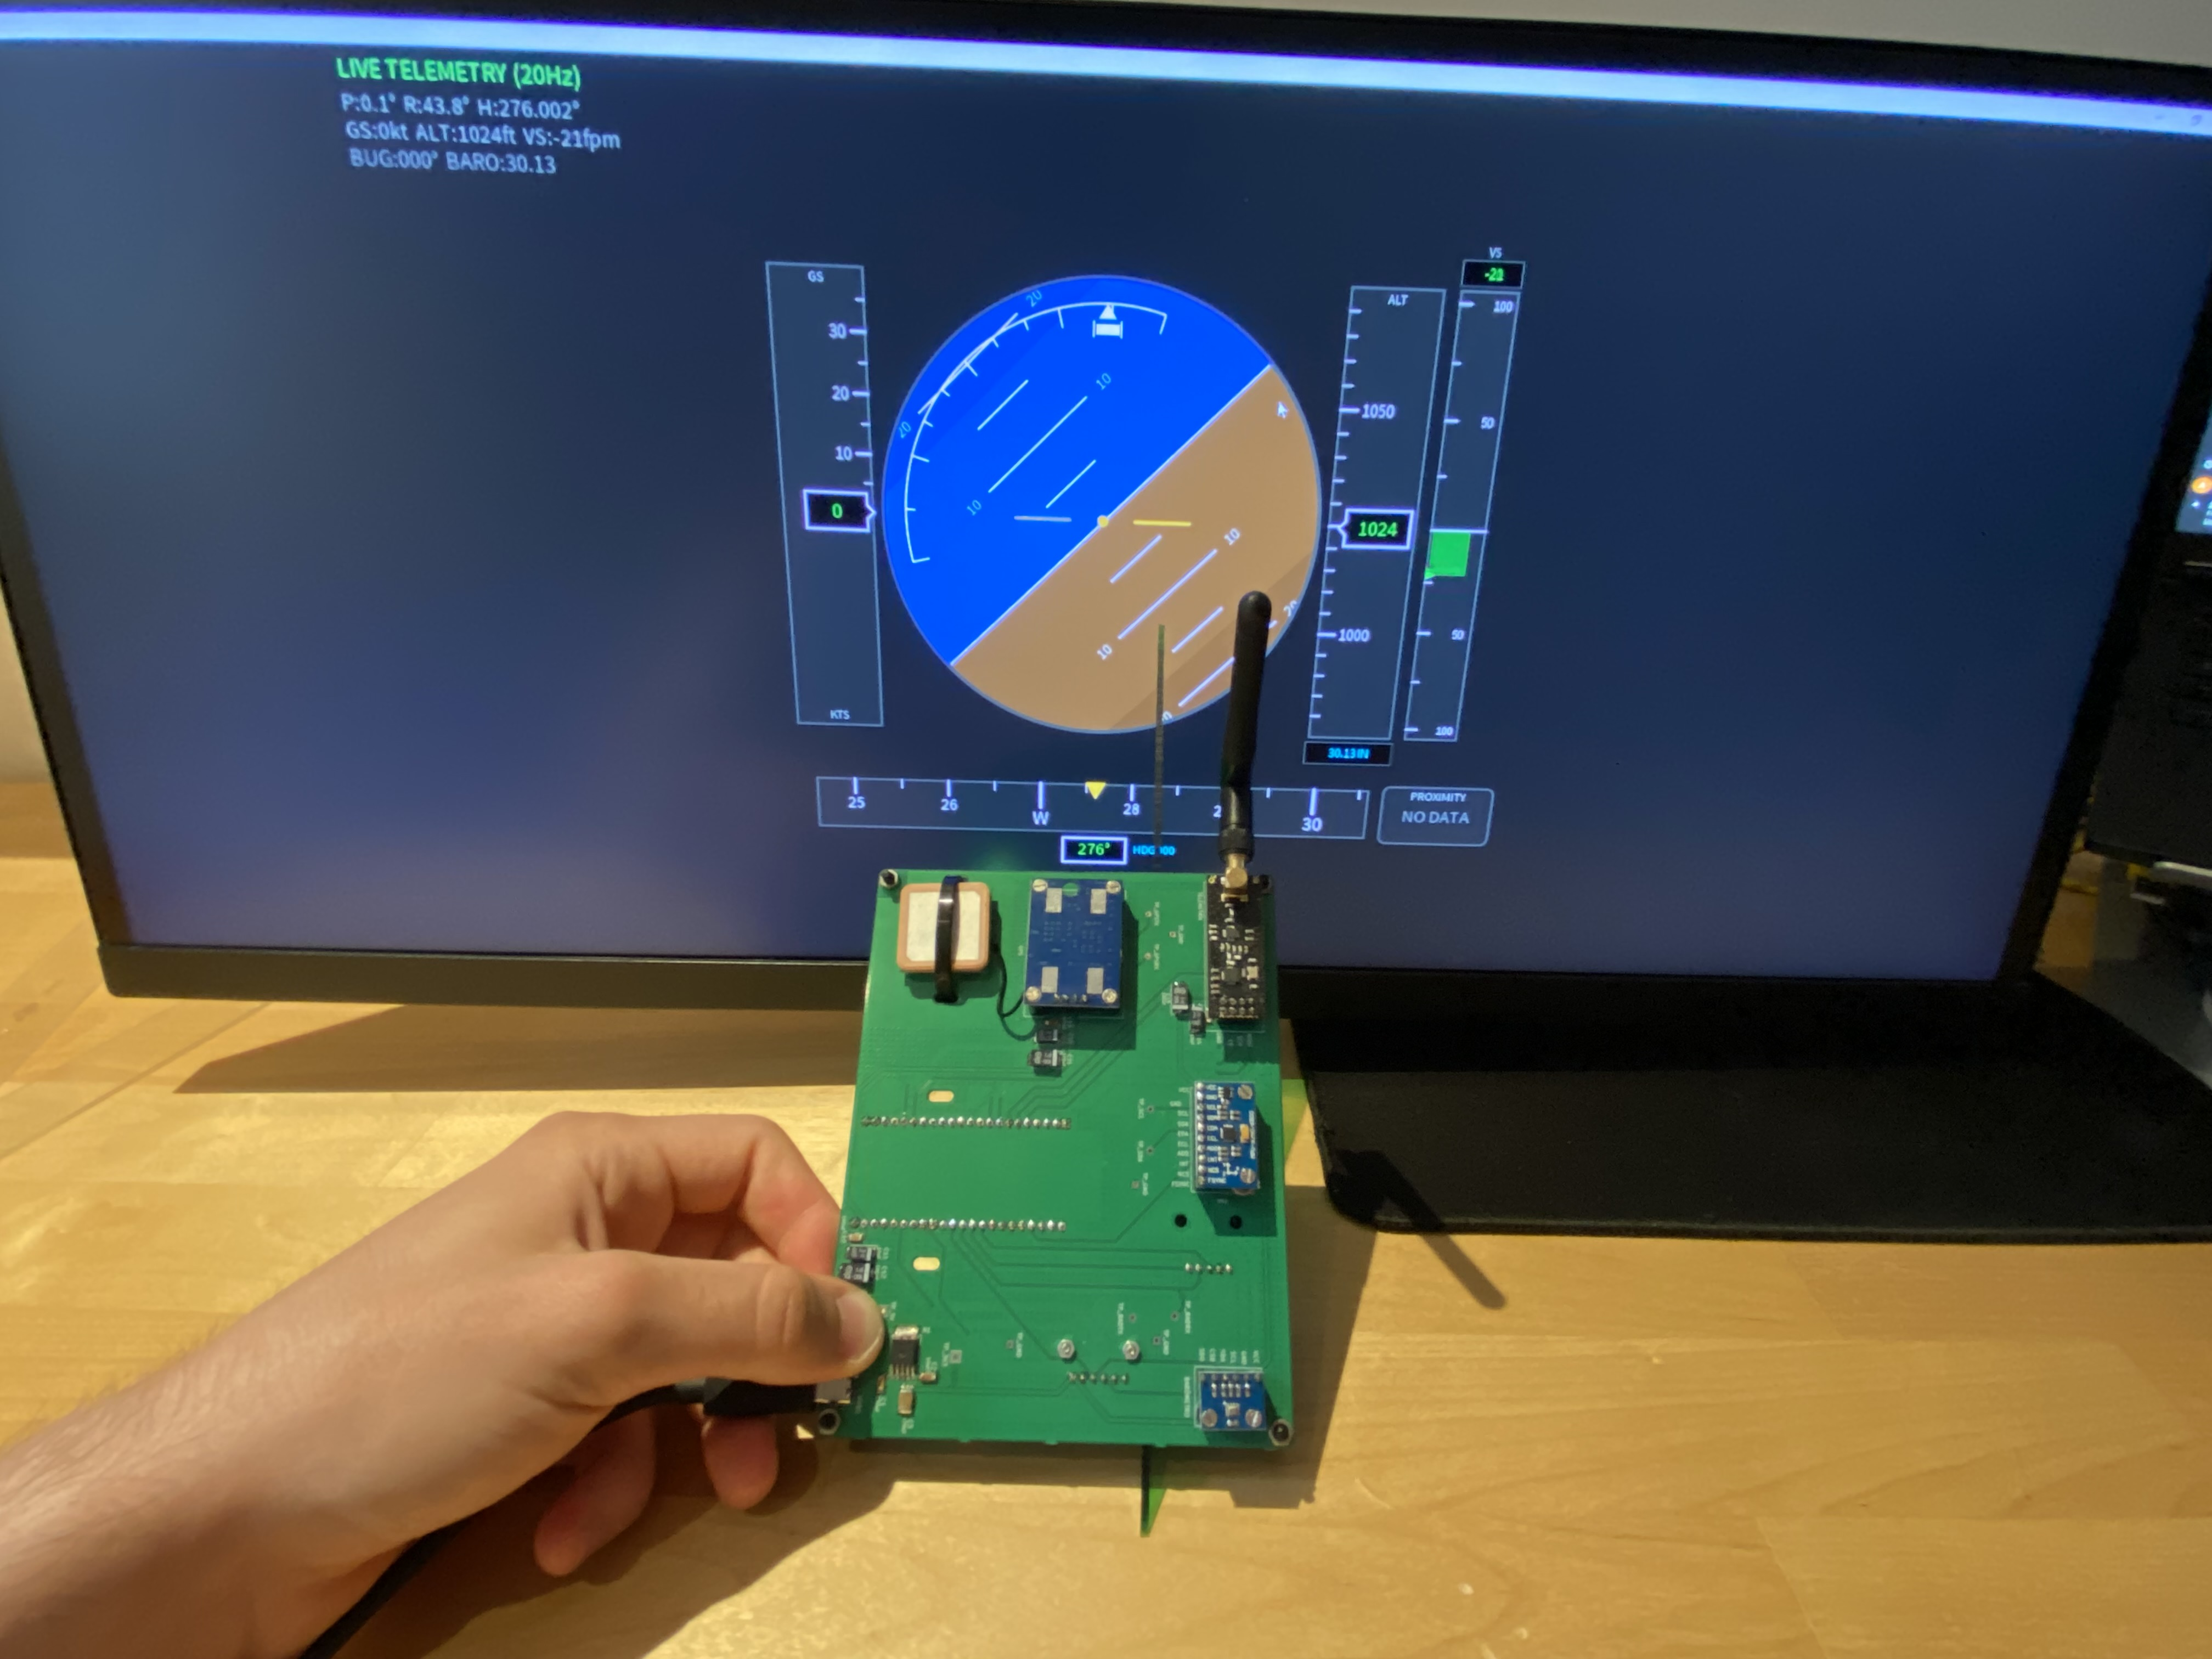
\includegraphics[width=0.6\linewidth]{Figures/IMG_2157.jpeg}
    \caption{Montaje para la medida de precisión de actitud con escuadra de
             referencia.}
    \label{fig:val_actitud_escuadra}
\end{figure}


% ========================================================================
\section{Rumbo magnético}
\label{sec:val_rumbo}

El rumbo magnético se valida en interior con la referencia de un teléfono móvil, que incorpora su propia calibración
y fusión, en varias orientaciones repartidas alrededor de los $360^{\circ}$. En cada
orientación se registra el rumbo indicado por la plataforma y el indicado por el
teléfono, y se calcula su desviación (\cref{tab:val_rumbo}).

{
\footnotesize
\begin{longtable}{C{3.2cm} C{3.2cm} C{3.2cm}}
\caption{Comparación del rumbo de la plataforma frente a un teléfono móvil}
\label{tab:val_rumbo} \\

\toprule
\textbf{Plataforma ($^{\circ}$)} & \textbf{Teléfono ($^{\circ}$)} & \textbf{Desviación ($^{\circ}$)} \\
\midrule
\endfirsthead

% Encabezado para la segunda página (y siguientes)
\multicolumn{3}{c}{\tablename\ \thetable\ -- Continuación de la página anterior} \\
\toprule
\textbf{Plataforma ($^{\circ}$)} & \textbf{Teléfono ($^{\circ}$)} & \textbf{Desviación ($^{\circ}$)} \\
\midrule
\endhead

% Pie de página temporal si la tabla se corta
\midrule
\multicolumn{3}{r}{\textit{Continúa en la siguiente página...}} \\
\endfoot

% Pie de página final para la última página de la tabla
\bottomrule
\endlastfoot

% --- Datos ---
$4{,}5$ & $0$ & $+4{,}5$ \\
$13{,}5$ & $10$ & $+3{,}5$ \\
$23{,}5$ & $20$ & $+3{,}5$ \\
$33{,}5$ & $30$ & $+3{,}5$ \\
$44{,}5$ & $40$ & $+4{,}5$ \\
$53{,}5$ & $50$ & $+3{,}5$ \\
$63{,}5$ & $60$ & $+3{,}5$ \\
$74{,}5$ & $70$ & $+4{,}5$ \\
$83{,}5$ & $80$ & $+3{,}5$ \\
$94{,}5$ & $90$ & $+4{,}5$ \\
$102{,}5$ & $100$ & $+2{,}5$ \\
$112{,}5$ & $110$ & $+2{,}5$ \\
$122{,}5$ & $120$ & $+2{,}5$ \\
$131{,}5$ & $130$ & $+1{,}5$ \\
$141{,}5$ & $140$ & $+1{,}5$ \\
$151{,}5$ & $150$ & $+1{,}5$ \\
$161{,}5$ & $160$ & $+1{,}5$ \\
$170{,}5$ & $170$ & $+0{,}5$ \\
$179{,}5$ & $180$ & $-0{,}5$ \\
$189{,}5$ & $190$ & $-0{,}5$ \\
$199{,}5$ & $200$ & $-0{,}5$ \\
$205{,}5$ & $207$ & $-1{,}5$ \\
$209{,}5$ & $210$ & $-0{,}5$ \\
$219{,}5$ & $220$ & $-0{,}5$ \\
$229{,}5$ & $230$ & $-0{,}5$ \\
$240{,}5$ & $240$ & $+0{,}5$ \\
$249{,}5$ & $250$ & $-0{,}5$ \\
$259{,}5$ & $260$ & $-0{,}5$ \\
$269{,}5$ & $270$ & $-0{,}5$ \\
$280{,}5$ & $280$ & $+0{,}5$ \\
$288{,}5$ & $290$ & $-1{,}5$ \\
$300{,}5$ & $300$ & $+0{,}5$ \\
$309{,}5$ & $310$ & $-0{,}5$ \\
$321{,}5$ & $320$ & $+1{,}5$ \\
$332{,}5$ & $330$ & $+2{,}5$ \\
$341{,}5$ & $340$ & $+1{,}5$ \\
$353{,}5$ & $350$ & $+3{,}5$ \\

\end{longtable}
}

\begin{figure}[H]
    \centering
    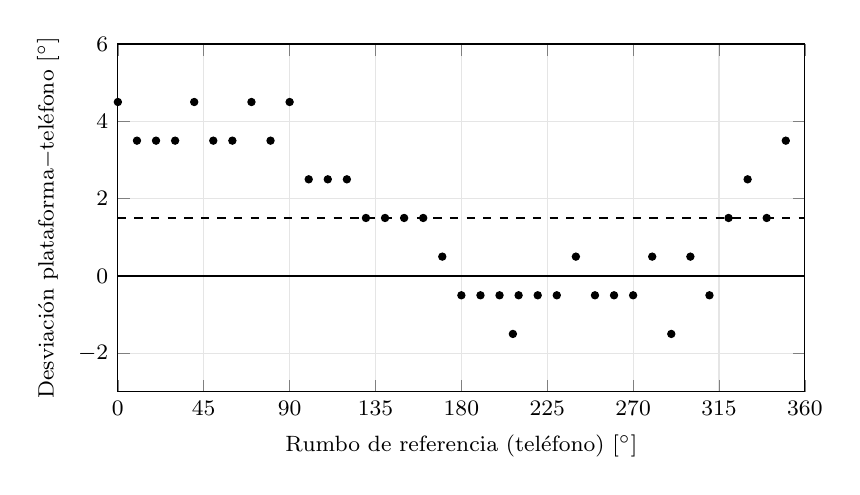
\begin{tikzpicture}
    \begin{axis}[
        width=0.85\linewidth, height=6cm,
        xlabel={Rumbo de referencia (tel\'efono) [$^\circ$]},
        ylabel={Desviaci\'on plataforma$-$tel\'efono [$^\circ$]},
        xmin=0, xmax=360, xtick={0,45,90,135,180,225,270,315,360},
        ymin=-3, ymax=6, grid=both, grid style={gray!20},
        tick label style={font=\footnotesize}, label style={font=\footnotesize},
    ]
    \addplot[only marks, mark=*, mark size=1.3pt] coordinates {
        (207,-1.5) (200,-0.5) (190,-0.5) (180,-0.5) (170,0.5) (160,1.5) 
        (150,1.5) (140,1.5) (130,1.5) (120,2.5) (110,2.5) (100,2.5) 
        (90,4.5) (80,3.5) (70,4.5) (60,3.5) (50,3.5) (40,4.5) (30,3.5) 
        (20,3.5) (10,3.5) (0,4.5) (350,3.5) (340,1.5) (330,2.5) 
        (320,1.5) (310,-0.5) (300,0.5) (290,-1.5) (280,0.5) (270,-0.5) 
        (260,-0.5) (250,-0.5) (240,0.5) (230,-0.5) (220,-0.5) (210,-0.5)
    };
    \addplot[dashed, domain=0:360, thick] {1.5};
    \addplot[domain=0:360] {0};
    \end{axis}
    \end{tikzpicture}
    \caption{Desviaci\'on del rumbo de la plataforma frente al tel\'efono. La l\'inea discontinua marca el
             sesgo medio residual ($+1{,}5^\circ$) tras la calibraci\'on.}
    \label{fig:val_rumbo_scatter}
\end{figure}

Estos resultados conviene analizarlos con cautela, ya que en interior existen múltiples interferencias que pueden afectar tanto a la plataforma como al teléfono. Por ello, esta comparación es más una verificación de la consistencia entre ambos magnetómetros que una medida exacta del norte verdadero. Aun así, los valores del teléfono se toman como buena referencia, y las desviaciones de la \cref{fig:val_rumbo_scatter} se mantienen dentro de márgenes aceptables.


% ========================================================================
\section{Precisión del posicionamiento GNSS}
\label{sec:val_gnss}

La precisión del posicionamiento se evalúa dejando la plataforma estática en
exterior, con vista despejada del cielo, y registrando la posición a \SI{5}{\hertz}
durante varios minutos. Sobre el conjunto de fijaciones se calcula la dispersión
respecto al centroide y, a partir de ella, el error circular probable (CEP).

Se obtiene un CEP50 de \SI{1.00}{\meter} y un CEP95 de \SI{1.86}{\meter}
(\cref{fig:val_gnss_scatter}). Ambos valores quedan por debajo del objetivo de
\SI{2.5}{\meter} de CEP fijado por RP05, que toma como referencia la cifra de la
hoja de datos del NEO-6M \cite{ds_neo6}. La retícula que se aprecia en la
distribución corresponde a la cuantización de la posición en la telemetría
(resolución de aproximadamente \SI{0.42}{\meter} por bit, \cref{sec:fw_word}); dado
que la dispersión real de las fijaciones, del orden de \SI{2}{\meter}, es muy
superior a ese paso, la cuantización no condiciona el valor del CEP obtenido.

\begin{figure}[H]
    \centering
    \includegraphics[width=0.7\linewidth]{Figures/val_gnss_scatter.png}
    \caption{Dispersión del posicionamiento GNSS en estático, con los círculos de
             CEP50 (\SI{1.00}{\meter}) y CEP95 (\SI{1.86}{\meter}).}
    \label{fig:val_gnss_scatter}
\end{figure}



% ========================================================================
\section{Precisión del sensor de distancia al suelo}
\label{sec:val_distancia}

La medida de distancia al suelo (RF06) se evalúa frente a distancias de
referencia conocidas, medidas con una cinta métrica. La plataforma se sitúa a
distintas alturas sobre una superficie plana (\SI{10}{\centi\meter},
\SI{20}{\centi\meter}, \SI{50}{\centi\meter} y valores adicionales) y se registra
la distancia indicada por el sensor de tiempo de vuelo VL53L1X, que es la fuente
activa del indicador de proximidad (\cref{sec:fw_proximidad}). La
\cref{tab:val_distancia} recoge las medidas; el error máximo del ToF es de
\SI{1.9}{\centi\meter}, coherente con la precisión de la hoja de datos
\cite{ds_vl53l1x}.

El radar HLK-LD2410C se incluye en la telemetría como segunda fuente, pero su
salida es una clasificación por puertas de distancia, no una medida métrica
estable, por lo que no se contrasta cuantitativamente; su papel es comparativo y
docente, según lo justificado en la \cref{sec:fw_proximidad}.

\begin{table}[H]
    \centering
    \caption{Precisión del sensor de distancia al suelo (VL53L1X)}
    \label{tab:val_distancia}
    \footnotesize
    \begin{tabularx}{\linewidth}{C{4.0cm} C{4.0cm} C{4.0cm}}
        \toprule
        \textbf{Ref.\ (\si{\centi\meter})} & \textbf{ToF medido (\si{\centi\meter})} & \textbf{Error (\si{\centi\meter})} \\
        \midrule
        $10$  & $10{,}3$ & $+0{,}3$ \\
        $20$  & $19{,}5$ & $-0{,}5$ \\
        $50$  & $51{,}2$ & $+1{,}2$ \\
        $100$ & $98{,}1$ & $-1{,}9$ \\
        \bottomrule
    \end{tabularx}
\end{table}


\section{Enlace de telemetría}
\label{sec:val_enlace}

La cobertura del requisito de alcance y fiabilidad del enlace (RP06) se justifica
por margen de diseño. El módulo NRF24L01+PA/LNA seleccionado (\cref{sec:enlace})
presenta un alcance en interior del orden de \SI{100}{\meter}, muy por encima de
las distancias de uso en laboratorio (unos pocos metros, con posibilidad de un
tabique intermedio), por lo que el enlace opera con holgura en el escenario
previsto. Como apoyo a la operación, el receptor emite cada segundo una sentencia
de estadística (\texttt{\$STATS}: paquetes recibidos y un porcentaje de pérdida
estimado a partir de las palabras de estado, a \SI{5}{\hertz}). Se trata de un
indicador de salud del enlace para supervisión en tiempo de ejecución, no de una
medida validada de pérdida de paquetes.


% ========================================================================
\section{Tasas de actualización y latencia}
\label{sec:val_latencia}

\paragraph{Tasa de refresco del PFD (RP02).}
El PFD se redibuja con el motor P2D a \SI{60}{FPS}, valor fijado por configuración
y muy por encima del mínimo de \SI{30}{FPS} de RP02.

\paragraph{Tasa de actualización de actitud (RP03).}
La fusión de actitud se ejecuta a \SI{100}{\hertz} y la actitud se transmite a
\SI{20}{\hertz}; ambas cadencias quedan fijadas por el planificador cooperativo
del firmware y superan el mínimo de \SI{20}{\hertz} de RP03.

\paragraph{Latencia extremo a extremo (RP01).}
La latencia extremo a extremo se acota analíticamente mediante el presupuesto de
retardos de transporte de la cadena, recogido en la \cref{tab:val_latencia}.

\begin{table}[H]
    \centering
    \caption{Presupuesto de latencia extremo a extremo (peor caso)}
    \label{tab:val_latencia}
    \footnotesize
    \begin{tabularx}{\linewidth}{X l}
        \toprule
        \textbf{Etapa} & \textbf{Contribución} \\
        \midrule
        Muestreo inercial y fusión (\SI{100}{\hertz})                 & $\approx$ \SI{10}{\milli\second} \\
        Espera del \textit{slot} de telemetría (\SI{20}{\hertz})       & $\leq$ \SI{50}{\milli\second} \\
        Transmisión RF con reconocimiento (\num{250}~kbps, \SI{32}{\byte}) & $\approx$ \SI{2}{\milli\second} \\
        Decodificación y salida serie USB (\SI{115200}{\baud}, $\approx$\SI{70}{\byte}) & $\approx$ \SI{6}{\milli\second} \\
        Espera de fotograma (\SI{60}{FPS})                            & $\leq$ \SI{17}{\milli\second} \\
        \midrule
        \textbf{Total (peor caso)}                                    & $\approx$ \SI{85}{\milli\second} \\
        \bottomrule
    \end{tabularx}
\end{table}

El peor caso, de aproximadamente \SI{85}{\milli\second}, queda por debajo del
límite de \SI{200}{\milli\second} de RP01. La latencia típica es menor, ya que los
términos de espera (\textit{slot} de telemetría y fotograma) promedian
aproximadamente la mitad de su valor de peor caso. 


% ========================================================================
\section{Resumen de cumplimiento de requisitos}
\label{sec:val_resumen}

La \cref{tab:val_cumplimiento} consolida el resultado de la validación frente a
los requisitos de rendimiento. Los requisitos funcionales (RF01--RF09) quedan
cubiertos según la \cref{tab:val_funcional}.

\begin{table}[H]
    \centering
    \caption{Resumen de cumplimiento de los requisitos de rendimiento}
    \label{tab:val_cumplimiento}
    \footnotesize
    \begin{tabularx}{\linewidth}{l X l l}
        \toprule
        \textbf{ID} & \textbf{Objetivo} & \textbf{Resultado} & \textbf{Estado} \\
        \midrule
        RP01 & Latencia $<$ \SI{200}{\milli\second}            & $\approx$ \SI{85}{\milli\second}  & Cumple \\
        RP02 & Refresco PFD $\geq$ \SI{30}{FPS}                & \SI{60}{FPS}            & Cumple \\
        RP03 & Actitud $\geq$ \SI{20}{\hertz}                  & \SI{20}{\hertz}  & Cumple \\
        RP04 & Actitud $\pm 3^{\circ}$                & error máx.\ $1{,}8^{\circ}$ & Cumple \\
        RP05 & GNSS $\leq$ \SI{2.5}{\meter} CEP                & \SI{1.00}{\meter} CEP50 & Cumple \\
        RP06 & Alcance de decenas de metros en interior        & $\approx$ \SI{100}{\meter} & Cumple \\
        \bottomrule
    \end{tabularx}
\end{table}